\documentclass{beamer}
\usepackage[utf8]{inputenc}
\usepackage{amsmath}
\usepackage{hyperref}
\usetheme{Boadilla}
\usecolortheme{default}
\title{Alan Turing y El problema de la parada}
\author{Kevin Mateo Cárdenas}
\date{2023}
\logo{
\includegraphics[height=2 cm]{Escudo.png}}
\begin{document}
\maketitle
\AtBeginSection[]
{
  \begin{frame}
    \frametitle{Contenido}
    \tableofcontents[currentsection]
  \end{frame}
}
\section{Historia de Alan Turing}
\begin{frame}{Alan Turing}
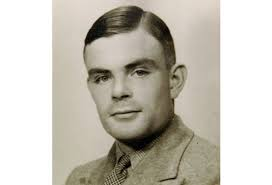
\includegraphics[scale=0.7]{turing.png}
\begin{itemize}
    \item Alan Mathison Turing fue un matemático, lógico, informatico teorico, criptógrafo, filósofo y biólogo teorico.\pause
    \item Nació el 23 de Junio de 1912 en Maida Vale, Londres.\pause
    \item Sus padres se llamaban Julius Mathison Turing y Ethel Sara Stoney
\end{itemize}
\end{frame}
\subsection{Su infancia}
\begin{frame}{Su infancia}
    \begin{center}
        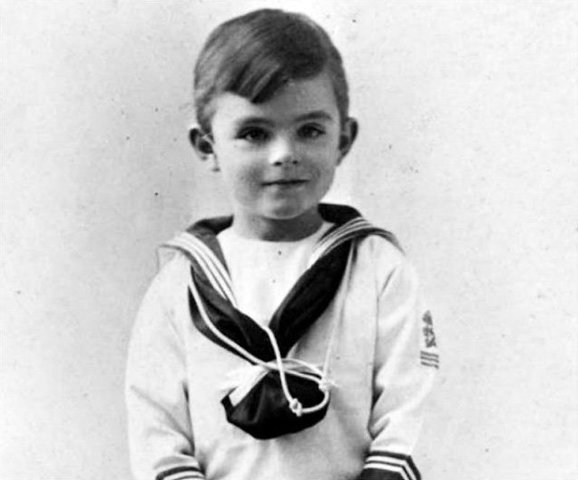
\includegraphics[scale=0.2]{turing0.png}
    \end{center}
\begin{itemize}
     \item vivió gran parte de su infancia en la india ya que su padre trabajaba en la administración colonial del pais.\pause
    \item mostró gran interés por la lectura, los rompecabezas y los números.\pause
    \item a sus 8 años tenía tal interés por el conocimiento y la experimentación quimica que diseño y construyó un pequeño laboratorio en casa. 
\end{itemize}

\end{frame}
\subsection{Su educación}
\subsubsection{Primeros pasos}
\begin{frame}{Su educación}
    \begin{itemize}
        \item Entre 1922 y 1926 estudió en la preparatoria Hazelurst, en la localidad Frant del condado de Sussex Oriental en Inglaterra, que tiene hoy una población estimada de 750 habitantes .\pause
        \item en 1926, a la edad de 13 años, ingresó en  \href{https://hmong.es/wiki/Sherborne_School}{el internado de Sherbone} en Doset Inglaterra. Se cuenta que en su primer día de clases en el internado coincidión con una \href{https://artsandculture.google.com/entity/m0hys9?hl=es}{huelga general en Inglaterra} pero su determinación por estudiar era tan grande que recorrió en su bicicleta los más de 96 Km que hay entre Southhantom y su escuela.
    \end{itemize}
\end{frame}
\begin{frame}{Su educación}
    \begin{itemize}
        \item La inclinación natural de Turing hacia la matemática y la ciencia no le atrajo el respeto de sus profesores de Sherborne, cuyo concepto de educación hacía mayor énfasis en los clásicos.\pause
        \item  En la escuela de Sherbone, ganó la mayor parte de los premios matemáticos que se otorgaban y, además, realizaba experimentos químicos por su cuenta aunque la opinión del profesorado respecto a la independencia y ambición de Turing no era demasiado favorable.\pause
        \item A pesar de ello, Turing continuó mostrando una singular habilidad para los estudios que realmente le gustaban, y llegó a resolver problemas muy avanzados para su edad (16 años) sin ni siquiera haber estudiado cálculo elemental.
    \end{itemize}
\end{frame}
\subsubsection{Christopher Morcom}
\begin{frame}{Christopher Morcom}
    \begin{center}
        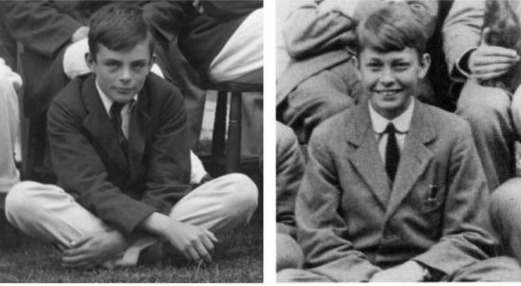
\includegraphics[scale=0.3]{Morcom.png}
    \end{center}
    \begin{itemize}
        \item \href{https://culturacientifica.com/2017/06/21/el-teorema-de-morcom/}{Christopher Morcom (1911, 1930)} estudió junto con Turing en la escuela de Sherborne y ambos compartían la pasión por la ciencia, Durante sus clases intercambiaban notas.\pause
        \item Christopher fue el primer amor de Turing, aunque no correspondido.\pause
        \item Su relación sirvió de inspiración para los esfuerzos futuros de Turing, pero fue interrumpida por la temprana muerte de Morcom, en febrero de 1930, por complicaciones de la tuberculosis bovina, contraída después de beber leche de vaca infectada algunos años antes.
\end{itemize}
\end{frame}
\begin{frame}{Christopher Morcom}\pause
    \begin{itemize}
        \item El evento causó gran pesar a Turing, quien lidió con su dolor trabajando mucho más duro en los temas de ciencias y matemáticas que había compartido con Morcom. En una carta a la madre de Morcom, Frances Isabel Morcom, Turing escribió:\pause\\
        \begin{center}
            "Estoy seguro de que no podría haber encontrado en ningún otro lugar a otro compañero tan brillante y, sin embargo, tan encantador y despreocupado. Consideraba mi interés en mi trabajo y en cosas como la astronomía (que él me presentó) como algo para compartir con él y creo que él sentía un poco lo mismo por mí ... Sé que debo poner tanta energía si no tanto interés en mi trabajo como si estuviera vivo, porque eso es lo que le gustaría que hiciera."
        \end{center}
    \end{itemize}
\end{frame}
\begin{frame}{Christopher Morcom}
    \begin{itemize}
        \item La relación de Turing con la madre de Morcom continuó mucho después de la muerte de Morcom, ella le enviava regalos a Turing y él le enviava cartas a ella, generalmente en los cumpleaños de Morcom.\pause
        \item Un día antes del tercer aniversario de la muerte de Morcom (13 de febrero de 1933), le escribió a la Sra. Morcom:\\\pause
        \begin{center}
            "Espero que estés pensando en Chris cuando esto te llegue. Yo también lo haré, y esta carta es solo para decirte que mañana pensaré en Chris y en ti. Estoy seguro de que está tan feliz ahora como cuando estuvo aquí. Tu cariñoso Alan."
        \end{center}
    \end{itemize}    
\end{frame}
\subsubsection{Su vida Universitaria}
\begin{frame}{Su vida universitaria.}
    \begin{itemize}
        \item Tuvo que ingresar en la escuela universitaria que eligió en segundo lugar, King's College, Universidad de Cambridge, en vez de en la que era su primera elección, Trinity,  pues por su falta de voluntad para esforzarse con la misma intensidad en el estudio de los clásicos que en el de la ciencia y la matemática, Turing suspendió sus exámenes finales varias veces.\pause
        \item Tras su graduación, se trasladó a la Universidad estadounidense de Princeton, donde trabajó con el lógico \href{https://es.wikipedia.org/wiki/Alonzo_Church}{Alonzo Church.}\pause
        \item alli también Recibió las enseñanzas de Godfrey Harold Hardy, un respetado matemático que ocupó la cátedra Sadleirian en Cambridge, y que posteriormente, fue responsable de un centro de estudios e investigaciones matemáticas entre 1931 y 1934.\pause
        \item En 1935 Turing fue nombrado profesor del King's College.
    \end{itemize}
\end{frame}
\subsection{Su aporte para ganar la segunda guerra mundial}
\begin{frame}{Sus aportes en la segunda guerra mundial.}
    \begin{itemize}
        \item El mundo está en deuda con Alan Turing, el genial matemático inglés que descifró los códigos que los nazis enviaban con su máquina Enigma.\\\pause
        \item Aunque gracias a su descubrimiento se salvaron millones de vidas, Turing tuvo que hacer frente a la intransigencia de su época, que lo convirtió en un paria y acabó con su vida.\pause 
        \item La reparación póstuma de su dignidad y su reconocimiento como científico llegarían demasiado tarde para él.
    \end{itemize}
\end{frame}
\begin{frame}{Sus aportes en la segunda guerra mundial.}
    \begin{itemize}
        \item El 3 de septiembre de 1939, Gran Bretaña entró en guerra con Alemania. En ese momento, Turing fue contratado como criptólogo por el ejército británico en Bletchley Park, una instalación militar ultrasecreta localizada en Buckinghamshire y conocida como Station X.\pause 
        \item La misión de Turing era intentar descifrar el sistema de cifrado de una máquina desarrollada por los nazis llamada Enigma, que el ejército polaco le había hecho llegar.\pause 
    \end{itemize}
    \begin{center}
        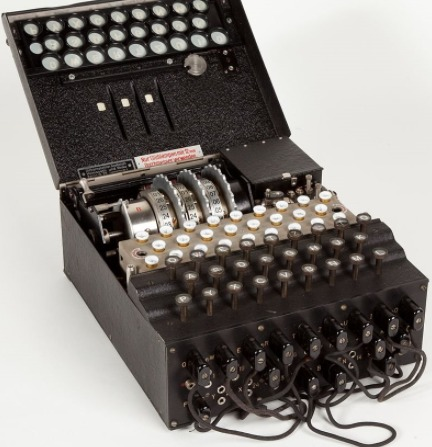
\includegraphics[scale=0.25]{enigma.png}
    \end{center}
\end{frame}
\begin{frame}{Maquina enigma}
    \begin{itemize}
        \item Enigma fue inventada por el ingeniero alemán Arthur Scherbius tras la primera guerra mundial.\pause
        \item Esta singular máquina generaba códigos basándose en el intercambio de signos. Su funcionamiento se basaba en enviar mensajes encriptados que alteraban la forma, pero no el contenido, con el objetivo de evitar que las encriptaciones fueran descifradas en caso de que estos mensajes fueran interceptados por el enemigo.
    \end{itemize}
    
\end{frame}
\subsection{Cusriosidades}
\begin{frame}{Cusriosidades} 
    \begin{itemize}
        \item En diciembre de 2011, William Jones y su miembro del Parlamento, John Leech , crearon una petición solicitando que el gobierno británico "perdonara" a Turing por su condena de "indecencia grave".\pause
        \item la petición decía: 
        \begin{center}
            "Pedimos al Gobierno de Su Majestad que conceda un indulto a Alan Turing por la condena de "indecencia grave". En 1952, fue declarado culpable de "indecencia grave" con otro hombre y se vio obligado a someterse a la llamada "organoterapia": castración química. Dos años más tarde, se suicidó con cianuro, con solo 41 años. Alan Turing fue llevado a una terrible desesperación y una muerte prematura por la nación por la que había hecho tanto por salvar. Esto sigue siendo una vergüenza para el gobierno británico y la historia británica. Un perdón puede ayudar de alguna manera a curar este daño. Puede actuar como una disculpa para muchos de los otros hombres homosexuales, no tan conocidos como Alan Turing, que fueron sometidos a estas leyes."
        \end{center}
    \end{itemize}
\end{frame}
\begin{frame}{Curiosidades}
    \begin{itemize}
        \item El 19 de agosto de 2014 sucedió algo excepcional. La reina Isabel II de Inglaterra proclamó finalmente el indulto póstumo a Alan Turing (1912–1954),condenado en 1952 por mantener relaciones homosexuales.\pause
        \begin{center}
            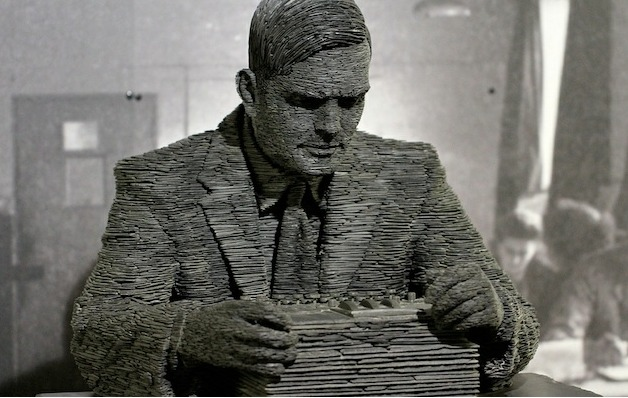
\includegraphics[scale=0.35]{indulto.png}
        \end{center}
    \end{itemize}
\end{frame}
\begin{frame}{Cusriosidades} 
\begin{itemize}
    \item El test Turing mide la capacidad de una máquina para hacerse pasar por un ser humano. Se realiza mediante una prueba conversacional entre un humano y una máquina. Si el ser humano es incapaz de distinguir entre ambos, se dirá que la máquina ha pasado dicho test , y podríamos considerar dicha máquina "inteligente".\pause
    \item En 2014 un bot computacional llamado Eugene Goostman fue capar de engañar a 30 de los 150 jueces a los que se sometió durante el test de Turing haciéndoles creer que estaban hablando con un niño ucraniano de 13 años.
\end{itemize}
\end{frame}

\section{El problema de la parada}
\begin{frame}{El problema de la parada}
El problema de la parada o problema de la detención para máquinas de Turing consiste en lo siguiente:\\\pause
\begin{center}
    Dada una Máquina de Turing $\mathbf{M}$ y una entrada $\mathbf{w}$, determinar si $\mathbf{M}$ terminará en un número finito de pasos cuando es ejecutada usando $\mathbf{w}$ como dato de entrada.
\end{center}
\pause
\begin{center}
        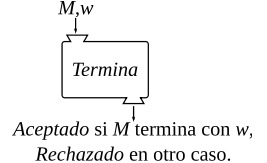
\includegraphics[scale=0.5]{problema0.png}
    \end{center}
\end{frame}
\subsection{Maquinas de turing}
\begin{frame}{Maquinas de turing}
    \begin{itemize}
        \item Llamamos Maqina de turing a $\mathbf{M}=(Q,\sum,\mathcal{T},B,F)$, donde:
        \begin{itemize}
            \item $Q$ es un conjunto \textbf{finito} de estados, que denotaremos por: $\{ q_0,q_1,...,q_n\}$\pause
            \item $\sum$ es el \textbf{alfabeto} el conjunto finito de simbolos de entrada.\pause
            \item $q_0$ es el \textbf{estado inicial}:
            El estado en el que se encuentra inicialmente la maquina.\pause
            \item F es el conjunto de estados finales\pause
            \item $\mathcal{T}$ es el conjunto de \textbf{símbolos de cinta}. el alfabeto es un subconjunto de $\mathcal{T}$\pause
        \end{itemize}
    \end{itemize}
    \begin{center}
        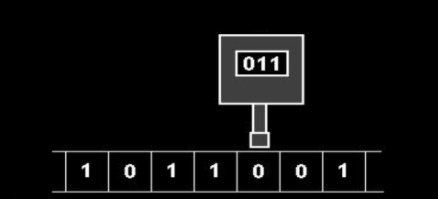
\includegraphics[scale=0.5]{maquina0.png}
    \end{center}
\end{frame}
\begin{frame}{Maquinas de Turing}
    \begin{itemize}
        \item para simplificar la teoría asumiremos sin perder generalidad que solo habran entradas en $\mathrm{N}^k$, $(n_1,n_2,...,n_k)$ y se verá de la forma: $(1,1..,1)_{(n_1+1)-veces},0,(1,...,1)_{(n_0+1)-veces},0,...,0,(1,...,1)_{(n_k+1)-veces}$
        que implica que su finción tien $k$ entradas.\pause
        \item el cabezal o lector de cinta inicia en el estado $q_0$ y en la posición que tenga el primer $1$ de izquierda a derecha.\pause
        \item los estados en una maquina tienen la forma $q_i=(x,y,F,q_j)\in Q$, donde $x,y\in\{0,1\}$ indica que el lector de la cinta se encentra en el estado $q_i$ leyendo $x$, el cual cambiará a $y$, se movera hacia $F\in\{R,L\}$, derecha o izquierda y pasará al estado $q_j$\pause
        \item y por último diremos que la maquina finalizará cuando el lector de cinta se encuentre en un estado $q_h\in Q$ leyendo $x\in\{1,0\}$ tal que la cinta tene a $\{1,0\}/\{x\}$ en esa posición.\\
        \item veamos un ejemplo.
    \end{itemize}
\end{frame}
\subsection{Equivalencia entre Maquinas de turing y funciones primitivas recursivas}
\begin{frame}{Funciones Recursivas Primitivas}
    \begin{itemize}
        \item Diremos que una función $h:\mathrm{N}^k\rightarrow\mathrm{N}$, es recursiva primitiva si:\pause
        \begin{itemize}
            \item para todo $k\in\mathrm{N}$ la función es nula de aridad $k$. o\pause
            \item es la función sucesor. o\pause
            \item es la función proyección $P_i^k$
            \item es una composición de funciones recursivas primitivas. o\pause
            \item la función sigue el suguente esquema de recursión:
            \begin{center}
                dadas f una función primitiva recursiva de aridad $k$, g una función recursiva primitiva de aridad $k+2$, y $h$ sea tal que:
                $$h(0,s\in\mathrm{N}^k)=f(s),$$
                $$h(suc(n),s)=g(h(n,s),n,s)$$
                donde $s\in\mathrm{N}^k$
            \end{center}\pause
        \end{itemize}
    \item se puede demostrar que el sistema de funciones recursivas primitivas es equivlente al sistema de maquinas de turing, es decir podemos computtar los mismos programs. Y diremos que un sistema computacional es una maquina universal de turing si su capacidad computacional es igual que la capacidad computacional de una maquina de turing.
    \end{itemize}
\end{frame}
\subsection{La irresolubilidad del problema}
\begin{frame}{El problema no se puede solucionar}
\begin{itemize}
    \item La irresolubilidad del problema se puede mostrar de varias formas, pero en esencia todas equivalen a un argumento diagonal de Cantor.\pause
    \item Supongamos que este problema sí se puede resolver algoritmicamente; entonces hay un programa, que llamaremos \textbf{Termina}, que cada vez que se le suministra el código de un programa p y sus datos de entrada $x$, hace un número finito de operaciones y responde $1$ cuando el programa termina o $0$ cuando el programa nunca termina.\pause
    \item Bajo la suposición de que existe este programa, se puede usar como subrutina de otro programa más grande, al que llamaremos \textbf{Diagonal} (en referencia a la diagonal de Cantor). 
\end{itemize}
\end{frame}
\begin{frame}{El problema no se puede resolver}
    \begin{itemize}
        \item Este programa recibirá como dato de entrada el código de un programa cualquiera \textbf{w}, y usará el programa \textbf{Termina} para decidir si el programa w termina cuando se le suministra ella misma como entrada (no hay nada de raro en esto, pues en la práctica hay programas como los compiladores que pueden suministrarse a sí mismos como dato de entrada).\pause
        \item A continuación, \textbf{Diagonal} hace lo opuesto: Si w termina entonces Diagonal entra en un ciclo infinito y si w entra en un ciclo infinito entonces Diagonal termina.\pause
        \begin{center}
            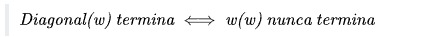
\includegraphics[scale=0.5]{diagrama.png}
        \end{center}
        \item recordemos que \textbf{Diagonal(w)}=\textbf{w(w)}, y vemos el absurdo.
    \end{itemize}
\end{frame}
\subsection{Marco histórico}
\begin{frame}{Historia del problema}
    \begin{itemize}
        \item Los conceptos de \textbf{algoritmo} y \textbf{computador} son definidos formalmente desde la informatica teorica por Alan Turing en su articulo "Sobre los números computables con una aplicación al problema de la decisión"\pause
        \item El problema de la desición fue resuelto en 1936 por Alonso church y Alan Turing de manera independiente, quienes demostraron que es imposible escribir dicho algoritmo.\pause
        \item el argumento de Turing se da por reducción al absurdo suponiendo la existencia de dicho algoritmo enfocado a decidir en la lógica de primer orden. llevandose este algoritmo a una maquina de turing, y concluyendo que este algoritmo es equivalente a un algoritmo que decide si una maquina para o no, cosa que él ya había mostrado que era imposible.
    \end{itemize}
\end{frame}
\begin{frame}{Historia del problema}
    \begin{itemize}
        \item Como consecuencia de los descbrimientos de las paradojas en la teoría de conjuntos se crearon las escuelas \textbf{\href{https://es.wikipedia.org/wiki/Logicismo}{logicista}, \href{https://es.wikipedia.org/wiki/Intuicionismo}{intuicionista}, y la \href{https://prezi.com/hnyrb4pzgznj/escuela-formalista-y-escuela-antiformalista/}{escuela formalista}}.\pause
        \item En 1900, en el congreso internacional de matemáticos, realizado en Paris, Francia. Hilbert (1862, 1943) propusó 23 problemas que marcarían el desarrolla de las matemáticas.\pause
        \item El décimo problema de estos problemas consistía en: ¿Es posible encontrar un procedimiento mecánico para calcular la solución de una clase párticular de ecuaciones diofanticas?.\pause
        \item El mismo Hilbert generalizo el problema y lo presentó en 1928 en el mismo congreso (esta vez realizado en Bolonia, Italia)\pause
    \end{itemize}
\end{frame}
\begin{frame}{Historia del problema}
    \begin{itemize}
        \item esta generalización es conocida actualmente como el problema de la desición.
        \item El resultado conocido hoy como \textbf{El teorema de incompletitud} de Gödel (1906, 1978) quien lo publicó en 1931 poniendo fin al ambicioso proyecto formalista de Hilbert.\pause
        \item el resultado de Gódel establece la insolución del problema de la desición en el caso particular de la veracidad o no de una fórmula en un sistema formal.\pause
        \item Lo más interesante de la solución del prolema de la decisión entregada por Turing fue que concibió la noción de \textbf{Computabilidad}, \pause
    \end{itemize}
\end{frame}
\section{Referencias}
\begin{frame}{Referencias}
    \begin{thebibliography}{}
        \bibitem{}{\href{https://www.euston96.com/alan-turing/}{Alan turing, Euston}}
        \bibitem{}{\href{https://es.wikipedia.org/wiki/Alan_Turing#Estudios}{Alan Turing, Wikipedia}}
        \bibitem{}{\href{https://culturacientifica.com/2017/06/21/el-teorema-de-morcom/}{El teorema de Morcom}}
        \bibitem{}{\href{https://historia.nationalgeographic.com.es/a/alan-turing-arma-secreta-aliados_16352}{alan turing, el arma secreta de los aliados. National Geographic}}
        \bibitem{}{Andrés Sicard Ramirez. Maquinas de Turing}
        \bibitem{}{\href{https://hmong.es/wiki/Alan_Turing}{Alan Turing, Wiki}}
        \bibitem{}{\href{https://www.matesfacil.com/automatas-lenguajes/Maquina-Turing.html}{Máquina de Turing, Wikipedia}}
        \bibitem{}{\href{https://es.wikipedia.org/wiki/Problema_de_la_parada}{Problema de la parada, Wikipedia}}
    \end{thebibliography}
\end{frame}
\end{document}
